\section{Reorganisation Projektstruktur}\label{sec:section-two}

Dieser Abschnitt befasst sich mit der Umstrukturierung des Projektverzeichnisses.

\subsection{Git-Repository}\label{subsec:subsection-two-one}

Das vorherige Semester war das erste mal, dass das Team eine Node JS Applikation entiwckelt hat.
Demnach wurde viel ausprobiert und es war noch kein Verständnis darüber vorhanden, wie eine solche Anwendung gut strukturiert aufgebaut wird.
Dieses Verständnis wurde über das letzte Semester aufgebaut und es wurde beschlossen, das Projekt neu zu strukturieren.
Dies kostete zum Anfang des Semesters viel Zeit, hat jedoch den Effekt, dass eine einheitliche Struktur aufgebaut wurde und die Implementierung neuer Funktionen einfach sind und einem fest definierten Standard folgen.

\subsubsection{Struktur des Projektstammverzeichnis (Project Root Path)}
In der efrsten Section wird auf die Gliederung in der ersten Ebene der Projektstruktur eingegangen, dem Project Root Path.
Während im vorherigen Semester eine Funktion meist alle komponenten, wie Responses, die Routendefinition und die eigentliche Funktionalität in einer Datei beinhalteten, wurden diese Dateien nun in drei einzelne Dateien aufgeteilt.
Dieses Vorhaben vergrößert das Repository um einiges, was die Dateianzahl angeht.
Daher muss sich eine geeignete Order-Struktur überlegt werden, um das Projekt trotz der Menge an Dateien übersichtlich zu gestalten.
Zunächst wurden alle Ordner und Dateien, die den eigentlichen Programmcode beinhalten, in einen Ordner namens \textit{src} abgelegt.
Dies hilft auch beim Bauen des Docker Images, da nun in der Dockerfile nur die Inhalte des src Ordners kopiert werden.
So wird kein unnötiger und ungewollter Overhead an Dateien in das Docker Image eingebaut.
Dateien wie \textit{.env}, die \textit{docker-compose.yaml} sowie der \textit{node_modules} Ordner gehören nicht mit in das Image, da sie unter anderem sensible Daten beinhalten, die jeder mit Zugriff auf das Docker Image einsehen kann.
Dies ist nicht gewollt, da die Docker Images öffentlich auf Docker Hub einsehbar sind.
Private Docker Image Repositories sind kostenpflichtig, weshalb sich gegen ihre Nutzung entschieden wurde.
Hier ist ein Vergleich der Projektstruktur nach dem letzten Commit des ersten Praxismoduls vs nach der Umstrukturierung in diesem Praxismodul:
\begin{figure}[h]
  \centering
  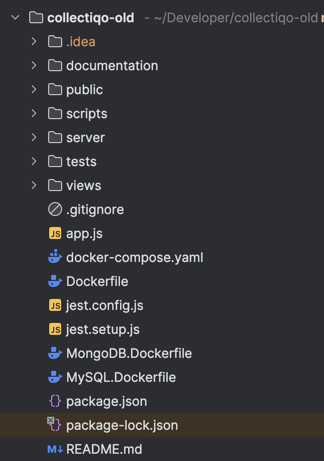
\includegraphics[width=0.5\textwidth]{root_path_structure_old}
  \caption{Old root path structure}
  \label{fig:root_path_structure_old}
\end{figure}
\begin{figure}[h]
  \centering
  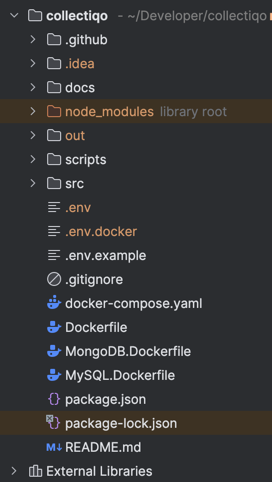
\includegraphics[width=0.5\textwidth]{root_path_structure_new}
  \caption{New root path structure}
  \label{fig:root_path_strucutr_new}
\end{figure}
Code, der zuvor unter den Ordnern Server, Public und Views zu finden war, wurde nun in den src Ordner verlagert.
Im nächsten Abschnitt wird der Inhalt des src Ordners genauer betrachtet.

\subsubsection{Struktur des Quellcodes}
Wie zuvor beschrieben beinhaltet der src Ordner jegliche Dateien, die den Quellcode der Collectiqo App beinhalten.
Hierzu zählen ebenfalls einige Ordner wie der public und views Ordner, die zuvor auf root Ebene vorhanden waren.
Hier eine Übersicht über alle Inhalte des src Ordners:
\begin{figure}[h]
  \centering
  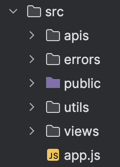
\includegraphics[width=0.5\textwidth]{src_folder_structure}
  \caption{src Folder Structure}
  \label{fig:src_folder_structure}
\end{figure}


Während zuvor alle bestandteile einer Funktion (Route, Response Codes und Funktionalität) in einer Datei gehandhabt wurden, wurden diese nun in drei seperate Dateien aufgeteilt.
Jede Route erhält eine eigene Datei, in welcher der Endpunkt für HTTP Request definiert wird und der entsprechende Controller aufgerufen wird.
Der Controller kümmert sich um den Aufruf der gewünschten Service Datei und handhabt die Response Codes, die beim Aufruf des Endpunkts zurück gegeben werden.
Die eigentliche Funktionalität ist in der Service Datei implementiert.
Diese Aufteilung bringt mehrere Vorteile mit sich.
Jede Funktionalität, die ab sofort implementiert wird, folgt genau diesem Muster, wodurch jede Implementierung für jedes Teammitglied klar nachverfolgbar ist.
Darüber hinaus erleichtert es das Debugging ungemein, da Probleme einfacher auf einzelne Bestandteile eines Funktionsaufrufs zurückgeführt werden können.
Kombiniert mit einer Ordnersturktur, die inhaltlich ferne Funktionen voneinander trennt, ist auf das navigieren innerhalb des Projets ereinfacht.
Schlusseindlich ist auch das Aufrufen vom HTTP Requests vereinfacht, da jeder Aufruf einheitlich ist.

\subsection{Docker Containerisierung}\label{subsec:docker-containerisierung}

Bereits im Praxismodul I wurde mit Docker Containern für die lokale Entwicklung gearbeitet.
Dieses Semester kamen zwei Aspekte hinzu, die auf dem angeeigneten Wissenstand aus dem vorherigen Semester aufgebaut haben - Multiplattform Images und das Deployen von Docker Anwendungen auf einem Server, der über das öffentliche Netz erreichbar ist.

\subsubsection{Multiplattform Images}\label{subsubsec:multiplattform-images}
Während der Durchführung des Projekts ist ein Teammitglied auf einen ARM-Prozessor umgestiegen.
Letztes Semester erfolgte die Programmierung ausschließlich auf x86 Windows Maschinen, wodurch Docker Images, die auf einer Maschine gebaut wurden, problemlos auf allen anderen Maschinen funktioniert haben.
Images, die für x86 Architektur gebaut wurden, funktionieren nicht auf ARM-Maschinen.
Eine Lösung wurde hier in Multiarchitektur Docker Images gefunden.
Wird ein solches Image aus einer Registry auf den eigenen Rechner gezogen, so erkennt Docker automatisch die Architektur, die benötigt wird.
So lässt sich bspw eine x86 und eine ARM Version des gleichen Docker Images in Docker Hub unter dem gleichen Registry Eintrag hosten.
Beim pullen des Images wird dann automatisch erkannt, für welche Architektur das Image benötigt wird.

Bevor die Images gehostet werden können, müssen diese aber zuerst gebaut werden.
Das Bauen von Multiarchitektur Images erfolgt mit einer Komponenten von Docker, die sich buildx nennt.
Buildx selbst ist hierbei eine Anwendung, die selbst in einem Docker Container läuft.
Damit interagiert wird über den üblichen docker build befehl, welcher nun aber um den buildx Befehl erweitert wird.
Das buildx Packet wird bei den aktuellsten Docker Versionen mitgeliefert, so muss der Container einfach wie folgt gestartet werden:

\lstset{language=Shell}
\begin{lstlisting}[label={lst:lst-shell-buildx-setup}]
docker buildx create --name multi-arch-build --use
\end{lstlisting}

Da verschiedene Images gebaut werden müssen, wurde folgendes Shell-Script entworfen, um den manuellen Aufwand zu verringern.
Übergeben werden hier der Name, den das Image tragen soll sowie die Dockerfile, die als Basis für das Image dienen soll.

\begin{lstlisting}[label={lst:lst-shell-buildx-build}]
#!/bin/bash

# Check if IMAGE_NAME is passed
if [ -z "$1" ]; then
  echo "Error: IMAGE_NAME is not provided."
  echo "Usage: $0 <image_name> <dockerfile_path>"
  exit 1
fi

# Check if DOCKERFILE_PATH is passed
if [ -z "$2" ]; then
  echo "Error: DOCKERFILE_PATH is not provided."
  echo "Usage: $0 <image_name> <dockerfile_path>"
  exit 1
fi

# Check if FULL_IMAGE_NAME is passed
if [ -z "$2" ]; then
  echo "Error: FULL_IMAGE_NAME is not provided."
  echo "Usage: $0 <image_name> <dockerfile_path>"
  exit 1
fi

IMAGE_NAME="$1"
DOCKERFILE_PATH="$2"
FULL_IMAGE_NAME="$3"

# Ensure you are logged in to the Docker registry
docker login || { echo "Docker login failed"; exit 1; }

# Build and push the Docker image
docker buildx build --platform linux/amd64,linux/arm64 -t ${FULL_IMAGE_NAME} -f ${DOCKERFILE_PATH} --push .
\end{lstlisting}

Die Push Flag am Ende des Befehls lädt gleichzeitig das neue Image in die Container Registry, in die der User eingelogt ist, hoch.
Im Fall dieses Projekts werden alle Images in Docker Hub gehostet.

\subsubsection{Deployment auf vServer}
Das hosten von den Docker Images in Docker Hub hat das Deployen auf den vServer sehr einfach gestaltet.
Bei dem Server handelt es sich um eine ARM-Maschine, spätestens hier wären also Multiplattform Images benötigt gewesen.
Zuerst wurde der ssh key des Servers als deploy Key auf GitHub hinterlegt.
Deploy Keys können pro Projekt hinterlegt werden und auf Read-Only geschaltet werden.
Sollten sich angreifer also einen Zugriff auf den Server verschaffen können, ist das Repository des Projekts somit vor ungewolltem löschen und überschreiben geschützt.
Mit anderen Repositories, die an den Account gebunden sind, kann nicht interagiert werden.
Das Repository wurde auf den Server geklont, da dieses die docker-compose.yaml Datei beinhaltet.
Um den Docker Compose Befehl ausführen zu können, muss jedoch eine Lese Berechtigung für die Docker Images im Docker Hub bestehen.
Hierzu wurde auf Docker Hub ein Token erstellt, mit Read-Only Berechtigungen, welchen zum Authentifizieren mit Docker Hub genutzt wurde.
Somit lassen sich die Images nun auf den Server pullen.
Die docker compose Datei sieht wie folgt aus:

\lstinputlisting[language=docker-compose, label={lst:docker-compose}]{../../../docker-compose.yaml}

Diese Verändert sich zur vorherigen Version insofern, dass sie nun auf Umgebungsvariablen für Werte wie Ports und Passwörter angewiesen ist.
Auch dem Container des NodeJS Servers wird eine .env Datei übergeben.
Da die .env Datei sensible, projektspezifische Daten beinhaltet, liegt im Repository nur eine Beispieldatei (.env.example), die nur den Key ohne die dazugehörige Value angibt.
Diese Datei wurde auf dem Server dann mit entsprechenden Values für die einzelnen Keys befüllt.
Schlussendlich wurde die docker-compose.yaml mit einem einfachen docker compose up ausgeführt, wodurch die Apps nun auf dem Server laufen.
Im nächsten Schritt soll das Deployment neuer Versionen der App automatisiert werden, da das Ausrollen einer neuen Version immer das manuelle ausführen der Docker Compose beinhaltet und ggf. das aktualisieren des Git Repositories.
